
\chapter{Vorgehensweise}

\section{Inferenz der Pose des Agenten}

\subsection{Datengewinnung}

Zur Erzeugung der Trainingsdaten wird in jedem \texttt{step}-Aufruf des Simulators das dazugehörige Kamerabild der DuckieBots abgegriffen, mit dem korrespondierenden Label versehen und anschließend abgespeichert. Das Label beinhaltet hierbei folgende Informationen:

\begin{enumerate}
	\item Kürzester Abstand $d$ zur rechten Fahrbahnmarkierung
	\item Winkeldifferenz $\Theta$ zwischen Orientierung des DuckieBots und der Fahrbahn
	\item Name der Kachelart, auf der sich der DuckieBot zur Zeit der Aufnahme des Kamerabildes befindet
\end{enumerate}

Es kann außerdem gesteuert werden, wie viele Kamerabilder aufgenommen werden sollen.
Im folgenden werden wir auf zwei verschiedene Ansätze eingehen, die wir zur Gewinnung der Daten verfolgt haben:

\subsubsection{Ansatz 1 - PID-Fahrt ohne Neuplatzierung des Agenten:}

Der DuckieBot wird mittels eines PID-Reglers gesteuert, so dass er die Mitte der rechten Fahrspur hält und den Streckenverlauf der Fahrbahn verfolgt. Dabei wird der DuckieBot auf einer zufälligen befahrbaren Kachel der Umgebung platziert. Die Orientierung des DuckieBots  wird hierbei ebenfalls zufällig ausgewählt.

\subsubsection{Ansatz 2 - PID-Fahrt mit Neuplatzierungen des Agenten:}

Bei diesem Ansatz wird der DuckieBot ebenfalls mit Hilfe eines PID-Reglers (wie in Anstatz 1 beschrieben) gesteuert. Der Unterschied hierbei ist, dass der DuckieBot nach einer gewissen Anzahl von \texttt{step}-Aufrufen des Simulators neu platziert wird. Die Platzierung des DuckieBots erfolgt hierbei ebenfalls zufällig, nach dem im Ansatz 1 beschriebenen Verfahren. 

\subsection{Netzwerkarchitektur}

Unsere Netzwerkarchitektur besteht aus 12 Schichten: einer Normalisierungsschicht, fünf Faltunsschichten, 2 Dropoutschichten, einer Flattenschicht und drei Fully-Connected-Schichten.
Eine schematische Darstellung der Netzarchitektur ist in Abbildung \ref{network-architecture} dargestellt. \\

Das Netzwerk nimmt das  Kamerabild des DuckieBots als Eingabe entgegen, wobei das obere drittel des Kamerabildes entfernt wurde. Dies hat den Vorteil, dass somit nur die relevanten Informationen für das Netzwerk im Kamerabild enthalten sind, wodurch sich das Training des Netzwerks verbessert. Das Netzwerk verarbeitet dann das eingehende Kamerabild und liefert anschließend die geschätze Pose, bestehend aus dem kürzestem Abstand $d$ zur rechten Fahrbahnmarkierung sowie der Winkeldifferenz $\Theta$ zwischen Orientierung des DuckieBots und der Fahrbahn. \\ 

\subsection{Normalisierungsschicht}
Die Grundidee der Normalisierungsschicht besteht darin, die Ausgabe einer Aktivierungsschicht zu normalisieren, wodurch die Konvergenz während des Trainingsprozesses verbessert wird. \cite{tensorflow} \\

\subsection{Faltungsschichten}
Nach der Normalisierungsschicht folgen die einzelnen Faltungsschichten. Diese sind für die Extraktion von Bildmerkmalen zuständig. \\

Die erste Faltungsschicht nutzt hierbei 24 verschiedene Filter (Kernel) der Größe 5x5 mit einer 2x2 Schrittbreite (stride) unter der Berücksichtigung der Bildränder (padding). Als Aktivierungsfunktion wird die ELu verwendet. Des Weiteren wird ein L2-Kernel-Regularizer eingesetzt, damit das Overfitting des Modells minimiert wird \cite{tensorflow2}.  \\ 
Das 5x5 große Fenster fährt dann über das Eingabebild und wendet alle 24 Filter auf den momentanen Bildausschnitt an. Jeder dieser Filter konzentriert sich dabei auf ein bestimmtes Bildmerkmal. \\

Die zweite Faltungsschicht nutzt 36 verschiedene Kernel. Die restlichen Parameter sind identisch zur ersten Faltungsschicht. \\

Die dritte Faltungsschicht nutzt 48 verschiedene Filter. Auch hier sind die restlichen Parameter identisch zur ersten Faltungsschicht. \\

Die vierte Faltungsschicht nutzt 64 verschiedene Kernel der Größe 3x3 mit einer 1x1 Schrittbreite, jedoch werden hier die Bildränder nicht berücksichtigt. Die restlichen Parameter sind wieder identisch zur ersten Faltungsschicht. \\

Die fünfte und letzte Faltungsschicht ist identisch zur vierten Faltungsschicht.

\subsection{Flattenschicht}

Nach den Faltungsschichten folgt eine sogenannte Flattenschicht, die dafür zuständig ist, die mehrdimensionale Ausgabe der Faltungsschichten  in eine eindimensionale Repräsentation zu überführen. \cite{hhu}

\subsection{Dropoutschichten}

Zwischen der vierten und der fünften Faltungsschicht befindet sich eine Dropoutschicht, sowie nach der Flattenschicht. Die Droputschichten dienen zur Minimierung der Gefahr einer Überanpassung des Modells an die Trainingsdaten. Dabei wird beim Training des Modells eine vorher spezifizierte Anzahl von Neuronen ausgeschaltet, die dann im kommenden Berechnungsschritt nicht berücksichtigt werden. \cite{wiki2}

\subsection{Fully-Connected-Schichten}

Nach den Faltungsschichten folgen anschließend drei Fully-Connected-Schichten die uns schlussendlich die geschätzte Distanz $d$ und geschätzte Winkeldifferenz $\Theta$ liefern.

\begin{figure}[H]
	\centering
	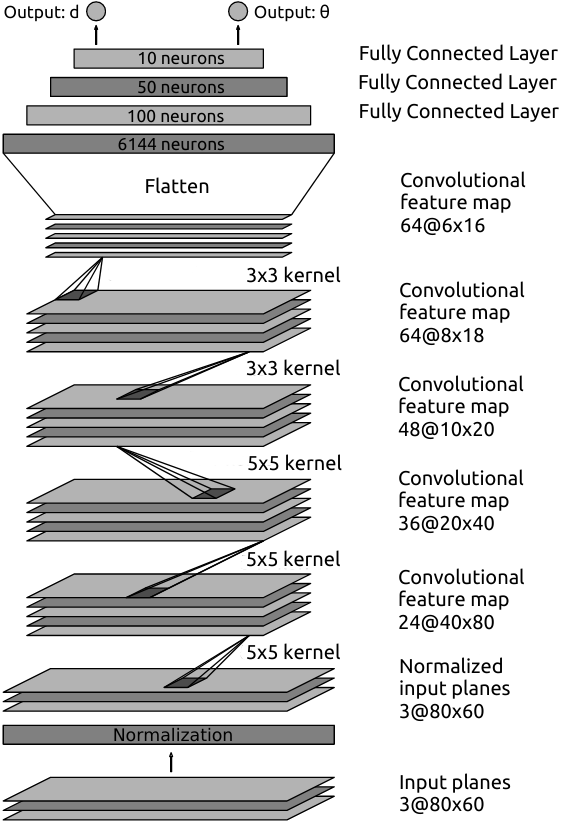
\includegraphics[width=0.56\textwidth]{kapitel4/images/network_architecture.png}
	\caption{Schematische Darstellung der Netzwerkarchitektur}
	\label{network-architecture}
	\vspace{0.2cm}
	\quelle\url{https://d3i71xaburhd42.cloudfront.net/0e3cc46583217ec81e87045a4f9ae3478a008227/5-Figure4-1.png}
\end{figure}

\section{Direkte Inferenz des Steuerbefehls}




